\section{Resultados e Discussões}
    
    Para testar o servidor foi preciso desenvolver um software cliente que se comunique com ele via rede TCP/IP, o qual, permite o usuário enviar os ângulos de referência de cada junta do robô e visualizar as leituras dos sensores de posição angular (\textit{encoder} absoluto de precisão) de cada junta em tempo real. 
    
    \begin{figure}[H]
        \centering
        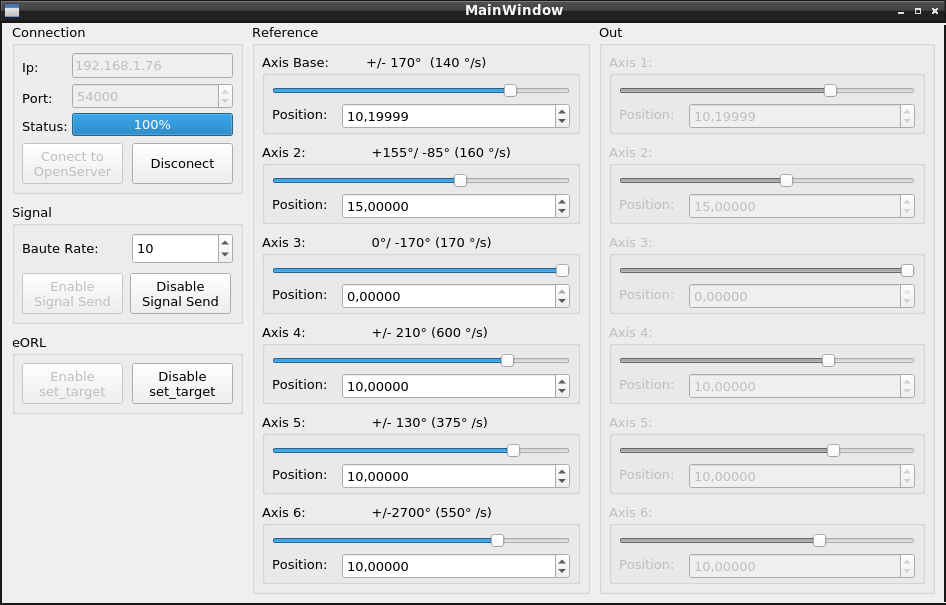
\includegraphics[width=\columnwidth]{imagens/Softwares/openclient_.png}
        \small 
        \centering 
        \caption{Software OpenClient em execução}
        \label{openclient_}
    \end{figure}
    
    Tal software foi chamado de \textit{OpenClientExemple}, escrito em C++ usando bibliotecas padrão do sistema operacional baseado em Linux, mas, que pode ser compilado para a arquitetura \textit{x86-64}, tendo sido executado em um computador pessoal convencional. Ele foi compilado também para \textit{Arm64} e executado em um \textit{Raspberry Pi 4}. Ambos testes foram realizados com sucesso, demonstrando que podem ser desenvolvidos programas clientes em outras arquiteturas.
    
    Além disso, foi testada a comunicação com o software \textit{Python}, usando a biblioteca padrão TCP/IP do mesmo, sendo executado no Sistema Operacional \textit{Windows} e também testada com um dispositivo móvel rodando \textit{Android}. A comunicação com o OpenServer foi realizada com sucesso, demonstrando que podem ser desenvolvidos softwares clientes em outros sistemas operacionais, inclusive para dispositivos móveis.
    
    A taxa de comunicação de um pacote a cada $2\,\mathrm{ms}$ (um pacote contendo todas as leituras ou posições das juntas), que foi aferida via cabo pode ser o suficiente para a maioria das aplicações, mas, essa taxa pode ser melhorada desenvolvendo-se uma forma mais eficiente de transmitir os dados. Por exemplo, criando uma nova modalidade que, de forma síncrona, envie dados ao mesmo tempo que recebe, ao invés de usar a forma assíncrona, que aguarda o recebimento de um dado para enviar o próximo. Outra possibilidade seria criar outra modalidade em que sejam transmitidos os dados binários direto da memória RAM, ao invés de convertê-los em \textit{strings} como foi feito nesse trabalho.
    
    A comunicação via rede sem fio também ocorreu a uma taxa de $2\,\mathrm{ms}$, com exceção de quando ocorria perda de dados devido à distância.
